%aias.tex
%%%\nisarcomm{merge, trim...move before example?}

    %Intelligent technology spans a wide spectrum of capabilities. With regards to autonomous systems, these 
    %Autonomous systems can describe anything from 
    %%a thermostat
    %a simple assembly line robot to the fabled HAL 9000. 
    While the main interest of the authors is geared towards human trust in `advanced' technology for dynamic robotic decision making under uncertainty, this survey we will take a more holistic view and use the term Artificially Intelligent Agent (AIA) to encompass a broad range of technologies that can be considered `autonomous'. 
    %%, to gather generally applicable insight. 
    An AIA is defined here as an agent that acts on an internally/externally generated goal, and possesses, to some extent, at least one of the capabilities shown in Fig.~\ref{fig:AIcapabilities} ~\cite{Russell2010-wv,Nilsson2009-rp,Luger2008-vf}. 
    While an AIA can describe anything from a simple assembly line robot to the fabled HAL 9000, this definition underscores the idea that many assurances that exist for one set of AIAs can be adapted and generalized for use in other AIAs. 
    %%For instance, chi-square consistency tests for Kalman filter state estimation algorithms for autonomous vehicle perception, target tracking and control systems \cite{Bar-Shalom2001-tg}. 
    In other words, this definition sets a scope for the bodies of research that are likely to have investigated assurances and assurance principles, which can be extended to any intelligent computing system. 
    The range of AIA capabilities also helps establish what kinds of assurances might be needed in future systems. 
    For example, assurances for an AIA that only carry out planning tasks will probably differ in design or implementation from assurances for an AIA that only carry out perception tasks. 
    
    %\nisarcomm{for me todo: one more important idea that hasn't been articulated here, but that we rely on from very first sentence of paper, is that AIA is seen as subordinate delegate to human -- this is key idea since it bridges definition of AIA to need for understanding user trust. can cite Chris Miller's work?}
    
    It should be noted that an AIA is assumed to operate with a degree of autonomy that is \emph{delegated} by a user. That is, an AIA is self-directed and self-sufficient in its task to the extent that the user's `intent frame' (desired goals, plans, constraints, stipulations and/or value statements) can be met by the AIA, regardless of how it actually accomplishes this. %or what intermediate decisions it needs to make to achieve these ends consistently. 
    Following \citet{Miller2014-av}, this view of autonomy as a delegation relationship refines need for `transparent AIAs' by avoiding a contradiction of purpose that stems from an otherwise naive interpretation. From a naive standpoint, one could argue that if AIAs are developed primarily in the first place to alleviate the burden of complex reasoning and other undesirable workloads by removing users from the task at hand entirely, then this purpose is undercut by exposure and explanation of sophisticated AIA inner workings to the user. 
    However, if AIAs are subordinates that are delegated tasks by users (who must still act as supervisors), the meaning of `transparency' shifts away from concern over how exactly an AIA accomplishes a task, towards concern over whether or not an AIA can execute the task as per the user's intent frame. 
    This delegation-based view naturally sets up the question of user trust in AIAs. 
    %
    %To this end, an artificially intelligent system needs to possess at least some of the capabilities shown in Figure~\ref{fig:AIcapabilities}~\cite{Russell2010-wv,Nilsson2009-rp,Luger2008-vf}. 
    %Some might argue that it is also necessary to add other categories like creativity and social intelligence~\cite{Tao2005-kh}. 
    %\brettcomm{SEEMS TO DETRACT---}Some of these categories are also not clearly separable; for instance, where does the capability to `plan' end, and `reasoning' begin? Nevertheless, these capabilities are conceptually useful in defining an AIA:     
%    \begin{description}
%        \item[Artificially Intelligent Agent (AIA):] an agent that acts on an internally/externally generated goal, and possesses, to some extent, at least one of the capabilities shown in Fig.~\ref{fig:AIcapabilities} ~\cite{Russell2010-wv,Nilsson2009-rp,Luger2008-vf}. .
%    \end{description}

	\begin{figure}[t!]%[thbp]
    	\centering
     	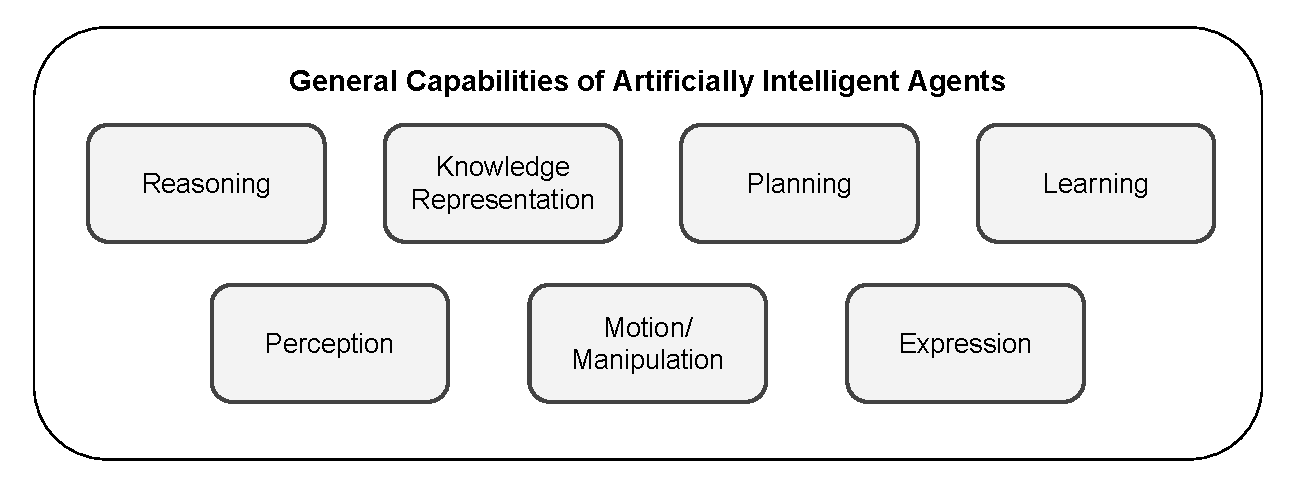
\includegraphics[width=0.55\textwidth]{Figures/AI_capabilities}
    	\caption{Set of possible AIA capabilities.}
        \label{fig:AIcapabilities}
    \end{figure}

%    The broad range of AIAs implied by this definition is most usefully viewed in terms of scope and adaptability. Scope refers to the range of possible applications for an AIA: does it have a small number of specialized application, or can it be used in many different applications? Adaptability refers to the ability of the AIA to become better at executing its goal over time. Low adaptability has often been associated with `weak AI' whereas high adaptability is often associated with `strong AI'.  Figure~\ref{fig:StrongWeak} depicts these axes for some (real and fictitious) AIAs.
%
%	\begin{figure}[htbp]
%    	\centering
%     	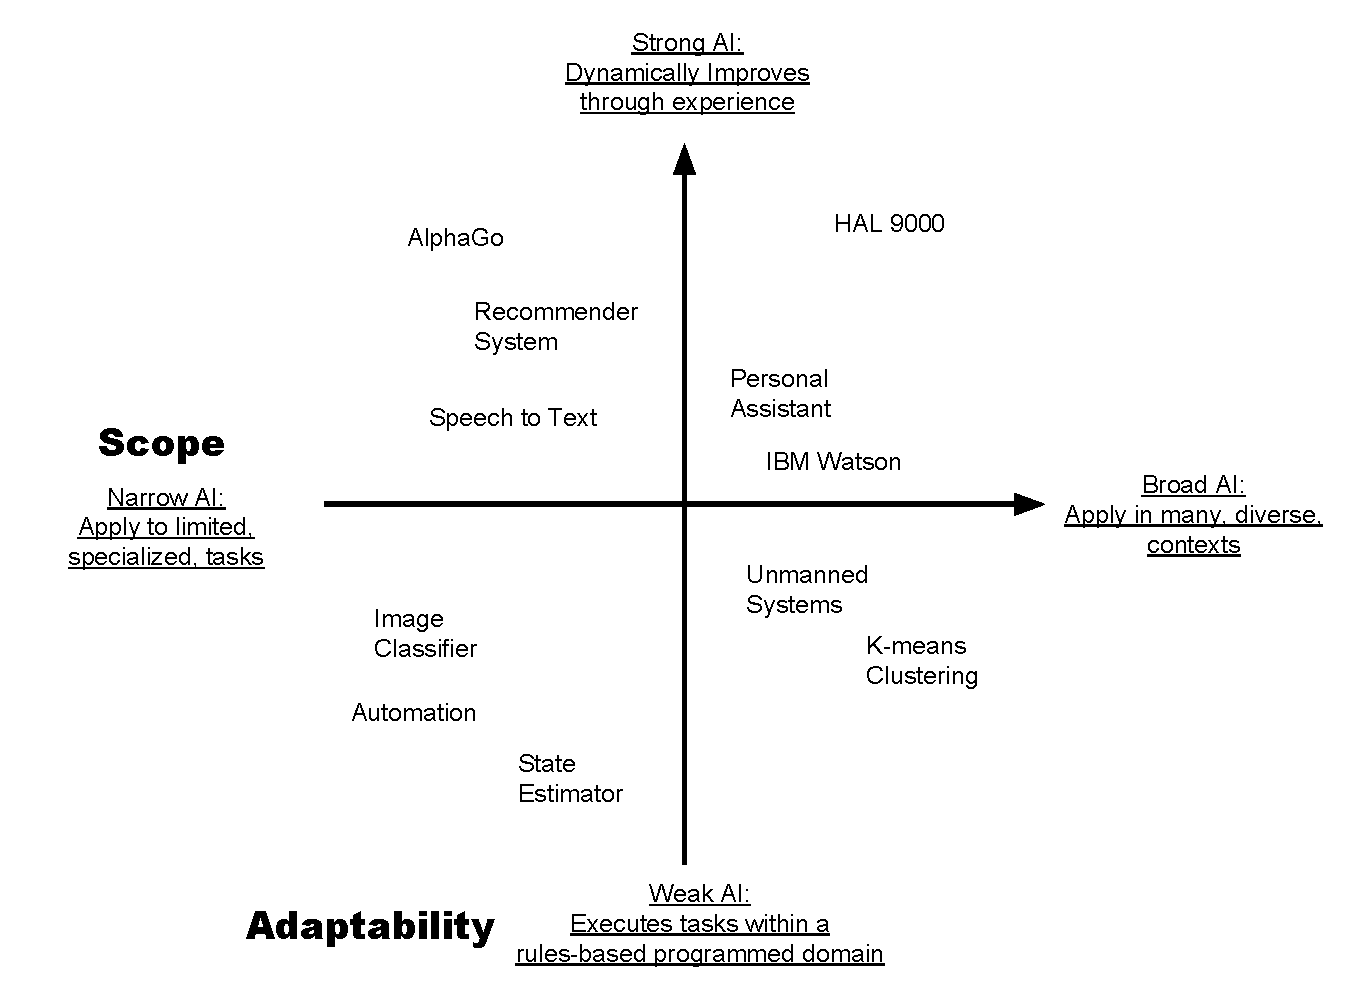
\includegraphics[width=0.7\textwidth]{Figures/strong_weak_narrow_broad.pdf}
%    	\caption{Illustration of the range of systems encompassed by the AIA definition. Horizontal axis reflects the scope of the AIA, the vertical axis reflects the adaptability of the AIA. \nisarcomm{todo: REMOVE}}
%        \label{fig:StrongWeak}
%    \end{figure}

%    Arguably, we might instead have used the term `artificial intelligence' (AI) instead of AIA. However, `AI' carries too much ambiguity (in its fullest meaning, it would possess all capabilities from Figure~\ref{fig:AIcapabilities}, and more). AIA allows the broad inclusion of \emph{any} system in the adaptability/scope plane. The research discipline of machine learning (ML) is a subset of the AI research landscape. Individual ML algorithms might be thought of as being a narrowly scoped AI that is contained within only one of the AIA capabilities. 
%
    %One might also question the need to define AIAs in the first place. 
    %This is to aid in the search for and understanding of assurances. As will be shown later, different methods of assurance can be found over the entire range of AIAs, so that an automation system such as a factory robot might be able to use similar assurances -- or more generally, similar principles of assurance -- as might a self-driving car, and vice-versa. The capabilities of AIAs (Fig.~\ref{fig:AIcapabilities}) are the sources of assurances; in other words, assurances cannot exist without some grounding set of AIA capabilities. 
%
 %   This definition %, while broad, is still useful because it 
 %   encompasses many systems that are typically described as `artificially intelligent'. 